\chapter{مفاهیم پایه و تجهیزات‌}

در این فصل به بررسی مفاهیم و تجهیزاتی که در این پروژه استفاده شده‌است می‌پردازیم. در هر بخش دلیل انتخاب خود را شرح می‌دهیم و آن را با سایر راه‌حل‌ها مقایسه می‌کنیم.

\section{حسگر}
همانطور که گفته‌شد برای پیش‌بینی نگهداری و عمر مفید تجهیزات نیاز به نظارت و جمع‌آوری اطلاعاتی راجع‌به این تجهیزات داریم. در این پروژه، اطلاعات جمع‌آوری‌شده مربوط به وضعیت لرزش تجهیزات است که با استفاده از حسگرهای لرزش \lr{MEMS} اندازه‌گیری می‌شوند.


در این پروژه تصمیم گرفتیم که بجای دما یا رطوبت از لرزش تجهیزات برای پیش‌بینی استفاده کنیم؛ زیرا لرزش برخلاف دو معیار دیگر بطور مستقیم شرایط عملیاتی تجهیزات را منعکس می‌کند که بیشتر بر اساس رفتارهای مکانیکی مانند چرخش موتور یا حرکت جریان در لوله ایجاد می‌شوند. هم‌چنین دو معیار دیگر وابستگی زیادی به محیط دارند اما لرزش تقریبا مستقل از عوامل خارجی است\cite{jung2017vibration}.


برای اندازه‌گیری لرزش دو نوع حسگر لرزش وجود دارد. حسگرهای مبتنی بر شتاب‌سنج \lr{MEMS} بر اکثر محدودیت‌های حسگرهای قدیمی مبتنی بر شتاب‌سنج پیزوالکتریک\LTRfootnote{Piezoelectric} غلبه می‌کنند. تفاوت این دو حسگر را می‌توان در \cref{sensor_comparison} \cite{jung2017vibration} دید.

\begin{table}[h!]
  \begin{center}
    \caption{مقایسه بین دو نوع حسگر مبتنی بر پیزوالکتریک و \lr{MEMS} \cite{jung2017vibration}}
    \label{sensor_comparison}
    \begin{tabular}{|c|c|c|} % <-- Alignments: 1st column left, 2nd middle and 3rd right, with vertical lines in between
    \hline
    	& پیزوالکتریک & \lr{MEMS}\\
    	\hline
    	قیمت (دلار) & +۳۰۰ & +۱۰\\
    	\hline
    	توان مصرفی ($mW$) & ۲۷ & ۳\\
    	\hline
    	اندازه (اینچ) & ۱/۹۷ × ۰/۹۸ × ۱ & ۰/۲ × ۰/۲ × ۰/۰۵\\
    	\hline
    	تراکم نویز ($\mu g$) & ۷۰۰ & ۴۰۰۰\\
    	\hline
    	بازه شتاب ($g$) & ۱۰ & ۱۰۰\\
    	\hline
    \end{tabular}
  \end{center}
\end{table}

بطور کلی حسگرهای نوع \lr{MEMS} ارزان‌تر، کم‌مصرف‌تر و کوچک‌تر هستند. در این پروژه حسگرها با باتری کار خواهند کرد و برای اندازه‌گیری به قطعات مورد نظر متصل می‌شوند. بنابراین کم‌مصرف‌بودن، ارزانی و کوچک‌بودن برای اتصال به بدنه ویژگی‌های مطلوبی است که در حسگرهای نوع \lr{MEMS} یافت می‌شود. \cref{fig:sensor} حسگر مدل \lr{ADXL 345} که در این پروژه استفاده کرده‌ایم.

\begin{figure}[!h]
\centering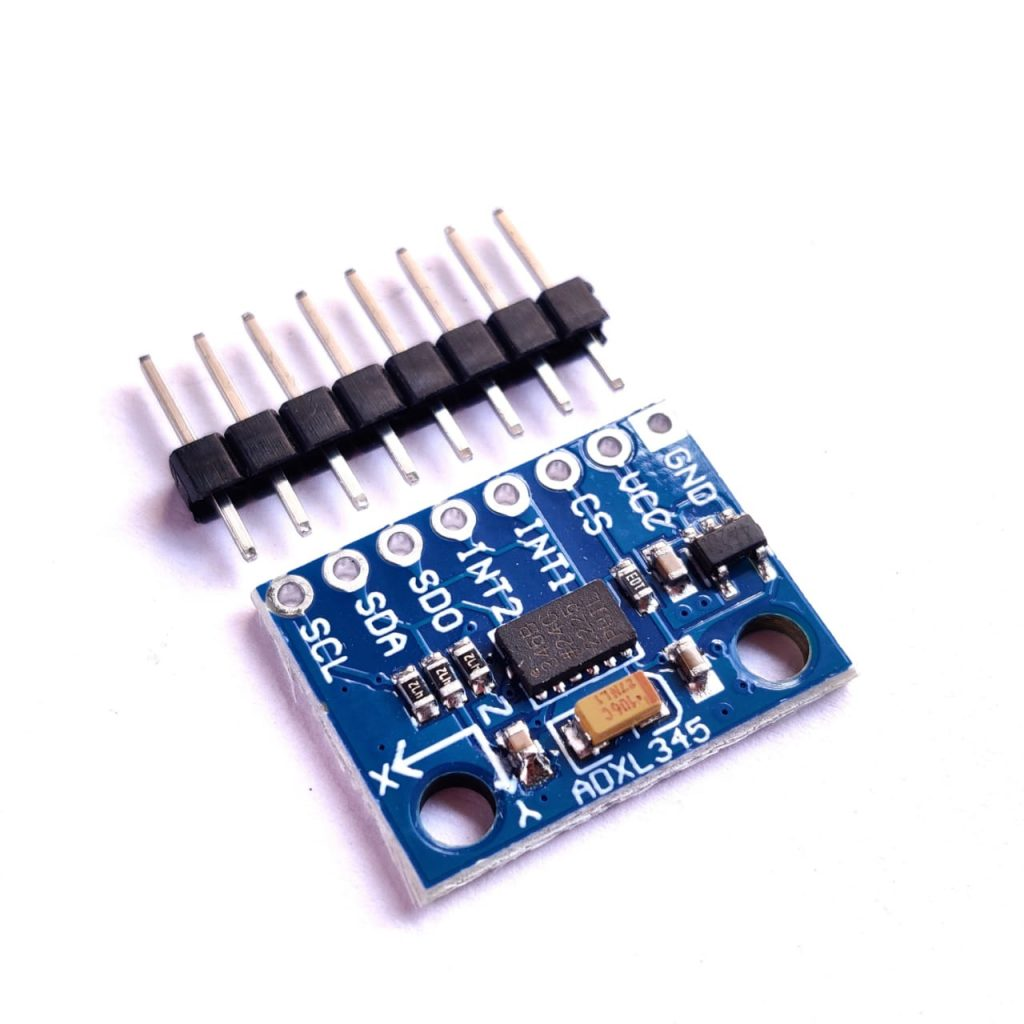
\includegraphics[scale=0.15]{sensor.png}
\caption{حسگر مدل \lr{ADXL 345}}\label{fig:sensor}
\end{figure}

این حسگر می‌تواند شتاب را در سه جهت، در چهار بازه قابل تنظیم ۲، ۴، ۸ و ۱۶ برابر گرانش با دقت‌های متفاوت اندازه‌گیری کند. خروجی این حسگر نیز با دو پروتکل \lr{SPI}\LTRfootnote{Serial Peripheral Interface} و \lr{I2C} قابل انتقال است.

\section{گره انتهایی}

برای کاهش بیشتر مصرف انرژی، دریافت اطلاعات حسگر و فرستادن آن برای دروازه به یک بورد\LTRfootnote{Board} نیاز داریم. بوردهای آردوینو\LTRfootnote{Arduino} اگرچه محدودیت‌هایی دارند، اما با توجه به ارزان‌بودن و برآورده‌کردن نیاز ما انتخاب مناسبی هستند. بورد استفاده‌شده در این پروژه آردوینو نانو است که در \cref{fig:arduino_nano} قابل‌مشاهده است. در این بورد از پورت سریال\LTRfootnote{Serial Port} برای ارتباط با ماژول زیگبی\LTRfootnote{Zigbee Module} و از پروتکل \lr{I2C} برای ارتباط با حسگر استفاده می‌کنیم. یکی از محدودیت‌های این بورد حافظه کم است که در نرخ‌های بالای نمونه‌برداری حسگر کار ما را سخت می‌کند که در فصل بعد بیشتر به آن می‌پردازیم.

\begin{figure}[!h]
\centering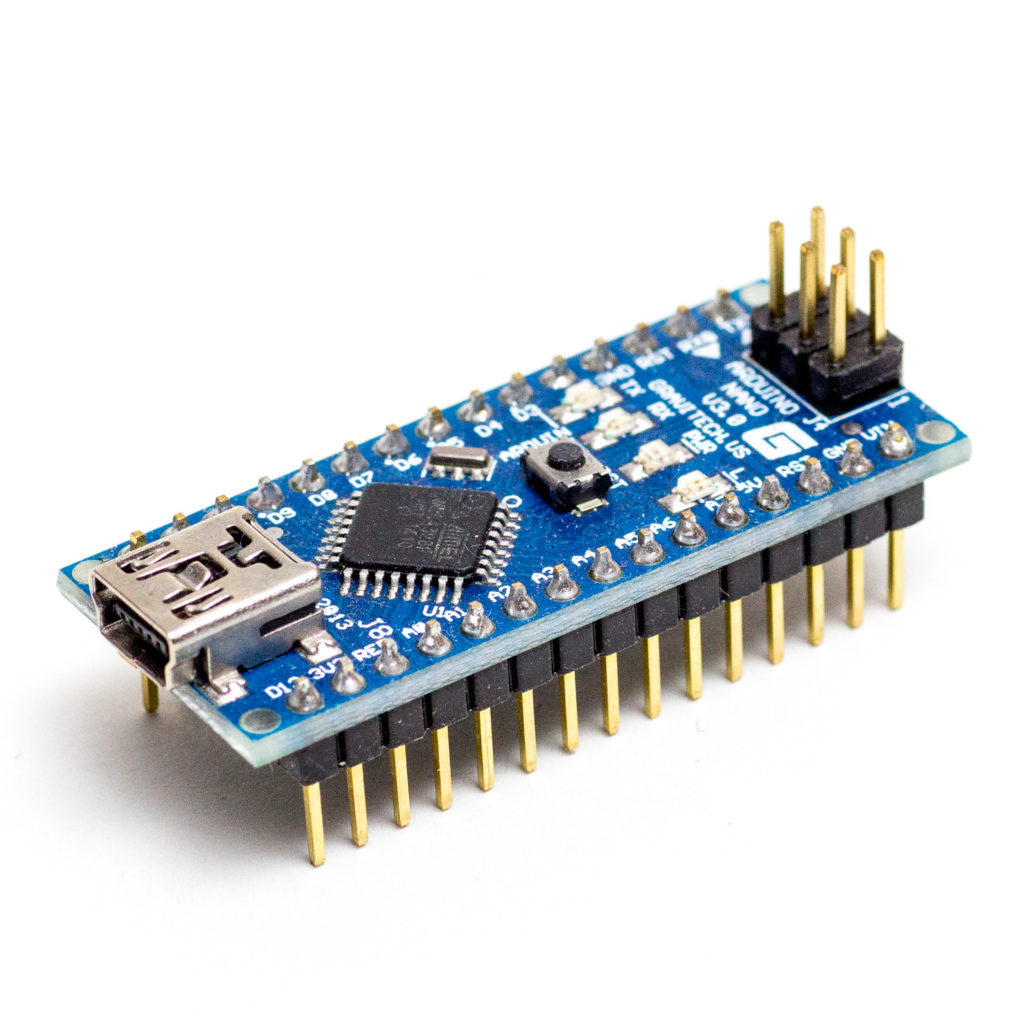
\includegraphics[scale=0.15]{arduino_nano.png}
\caption{بورد آردوینو نانو}\label{fig:arduino_nano}
\end{figure}

\section{پروتکل ارتباطی}

برای ارسال اطلاعات از گره‌های متصل به حسگر به دروازه نیاز به یک پروتکل ارتباطی داریم. نیازهای ما در رابطه با این پروتکل عبارتند از:
\begin{itemize}
\item کم‌مصرف‌بودن: با توجه به اینکه گره‌های ما به باتری متصل هستند، به پروتکلی نیاز داریم که در مصرف انرژی بسیار بهینه عمل کند تا بتوان بدون تعویض باتری اطلاعات را تا چند سال برای دروازه فرستاد.
\item پوشش و نفوذ سیگنال: در هر کارخانه یک دروازه نصب شده‌است، کارخانه‌ها مساحتی متوسط دارند و مانع خاصی نیز در آنها وجود ندارد. پس نیاز به پوشش یا قدرت نفوذ بالایی در سیگنال ارسالی نداریم.
\item توپولوژی\LTRfootnote{Topology}: با توجه به وجود یک دروازه و چندین گره که همگی اطلاعات را برای دروازه ارسال می‌کنند، نیاز به پروتکلی داریم که از توپولوژی ستاره پشتیبانی کند.
\item ارتباط مطمئن\LTRfootnote{Reliable Communication}: ارسال ناقص و یا از دست‌دادن اطلاعات حسگرها می‌تواند باعث پیش‌بینی اشتباه شود. بنابراین، به پروتکلی با قابلیت ارتباط مطمئن و کنترل خطا نیاز داریم.
\end{itemize}

در \cref{fig:protocol_comp} پروتکل‌های ارتباطی با معیارهای مختلف مقایسه شده‌اند. بر اساس ویژگی‌های موردنیاز پروتکل زیگبی انتخاب مناسب‌تری نسبت به سایر پروتکل‌ها است که در ادامه آن را معرفی می‌کنیم.

\begin{figure}
\centering
\begin{subfigure}{.5\textwidth}
  \centering
  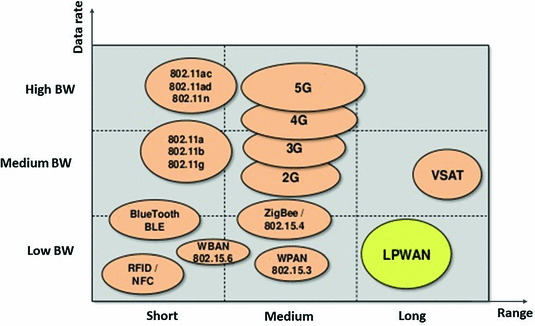
\includegraphics[height=5cm, width=.9\linewidth]{protocol_data_range.png}
    \centering
  \caption{مقایسه بر حسب نرخ داده و بازه پوشش \cite{carlsson2018measuring}}
\end{subfigure}%
\begin{subfigure}{.5\textwidth}
  \centering
  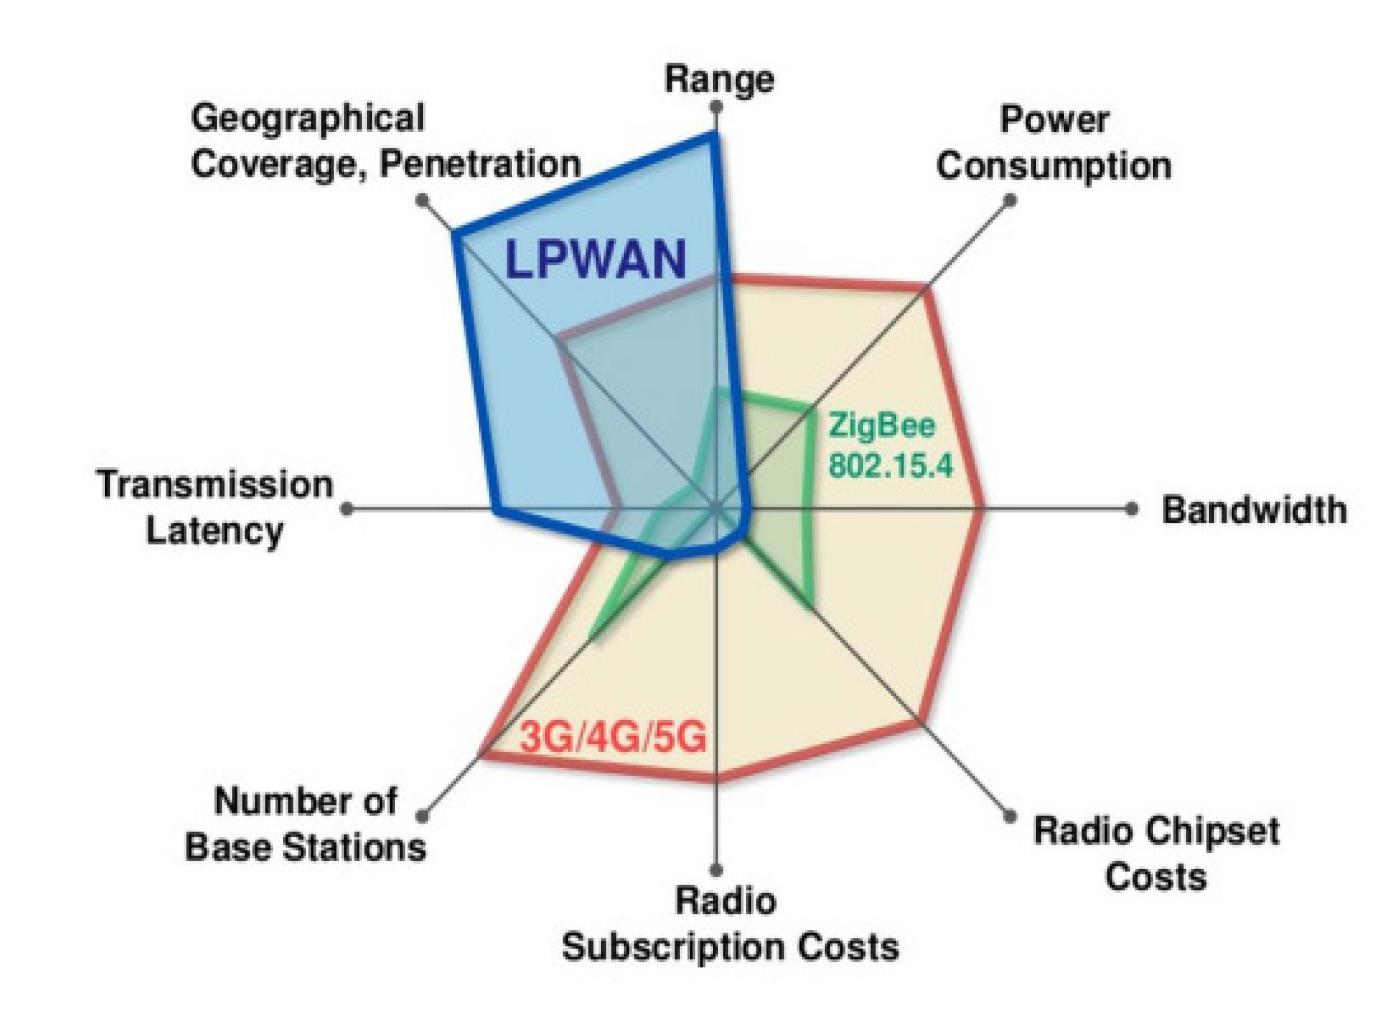
\includegraphics[height=5cm, width=.9\linewidth]{protocol_m_criteria.png}
    \centering
  \caption{مقایسه بر حسب انرژی، بازه پوشش، نفو‌ذ، تاخیر، هزینه و پهنای باند \cite{tabbane2017iot}}
\end{subfigure}
\caption{مقایسه پروتکل زیگبی و سایر پروتکل‌های اینترنت اشیاء}
\label{fig:protocol_comp}
\end{figure}

\subsection{استاندارد زیگبی}

زیگبی یکی از استانداردهای فرستنده-گیرنده\LTRfootnote{Tranceiver} در شبکه‌های حسگر بی‌سیم\LTRfootnote{Wireless Sensor Network} است که بصورت گسترده مورد استفاده قرار گرفته‌است. زیگبی بر روی \lr{IEEE802.15.4} مشخصات شبکه شخصی بی‌سیم با نرخ داده پایین\LTRfootnote{Low Rate Wireless Personal Area Network(LR-WPAN} را تعریف می‌کند تا بتواند از دستگاه‌های نظارتی و کنترلی با توان مصرفی و نرخ داده پایین پشتیبانی کند. زیگبی توسط اتحاد زیگبی\LTRfootnote{Zigbee Alliance} توسعه داده شده‌است؛ که صدها عضو دارد. اتحاد زیگبی لایه‌های شبکه، امنیت و برنامه و \lr{IEEE802.15.4} لایه‌های سخت‌افزار و کنترل دسترسی به رسانه\LTRfootnote{Media Access Control(MAC)} را تعریف می‌کنند\cite{ramya2011study}.

استاندارد شبکه بی‌سیم زیگبی جای خالی‌ای را در بازار پر می‌کند که توسط سایر شرکت‌ها نادیده گرفته شده‌است. 
اکثر استانداردهای بی‌سیم به دنبال نزدیک‌شدن به اینترنت و رسیدن به سرعت‌های بالاتر هستند. اما زیگبی در تلاش است تا با ارائه نرخ ارسال پایین‌تر انتظار مصرف انرژی پایین را برآورده کند. سایر استانداردها به دنبال افزودن ویژگی\LTRfootnote{Feature}های بیشتر و ارائه خدماتی نظیر استریم با کیفیت بالا\LTRfootnote{High-Definition Streaming} هستند؛ درحالیکه زیگبی با پشته\LTRfootnote{Stack}‌ای کوچک تنها هدف دارد که بتوان داده‌هایی با حجم کم و تعدد پایین مانند کنترل چراغ یا خواندن داده‌های سنسور دما را ارسال کرد\cite{gislason2008zigbee}.

\subsection{ویژگی‌های زیگبی}

\subsubsection{قابلیت اطمینان بالا}

ارتباطات بی‌سیم بطور کلی ارتباطات نامطمئنی هستند اما زیگبی در چند سطح قابلیت اطمینان بالایی فراهم می کند که عبارتند از:

\begin{itemize}
\item \lr{IEEE802.15.4}: در آن از ترکیبی از فناوری‌هایی مانند \lr{O-QPSK}\LTRfootnote{Offset-Quadrature Phase-Shift Keying} و \lr{DSSS}\LTRfootnote{Direct Sequence Spread Spectrum} استفاده می‌شود که کارایی بسیار خوبی در محیط‌های با نرخ سیگنال به نویز پایین دارند\cite{gislason2008zigbee}.
\item \lr{CSMA-CA}\LTRfootnote{Carrier Sense Multiple Access Collision Avoidance}: زیگبی از این فناوری برای کنترل دسترسی به رسانه استفاده می‌کند. قبل از ارسال زیگبی به کانال گوش می‌دهد. اگر کسی در حال ارسال نباشد، اطلاعات خود را ارسال می‌کند. این روند از تداخل اطلاعات فرستنده‌های محتلف و ایجاد نیاز برای ارسال دوباره جلوگیری می‌کند\cite{gislason2008zigbee}.
\item کنترل خطا: در هر فریم\LTRfootnote{Frame} زیگبی از \lr{CRC}\LTRfootnote{Cyclic Redundancy Check} ۱۶ بیتی بعنوان چک‌سام\LTRfootnote{Checksum} استفاده می‌شود که قابلیت تشخیص خطا در هر فریم را ایجاد می‌کند\cite{gislason2008zigbee}.
\item فریم تایید: هر فریم در کل ۴ بار برای مقصد ارسال می‌شود(۳ بار ارسال مجدد). اگر باز هم فریم نتواند ارسال شود به مبدا اطلاع داده می‌شود\cite{gislason2008zigbee}.
\end{itemize}

\subsubsection{مصرف انرژی پایین}

ماژول‌های زیگبی در مصرف انرژی بسیار بهینه هستند. یک شبکه زیگبی می‌تواند تا چند سال تنها با استفاده از باتری عمل کند. اگر استفاده از زیگبی به‌درستی مدیریت شود این زمان حتی می‌تواند به عمر باتری اگر بدون استفاده در قفسه بماند برسد. دلیل این استفاده کم این است که گره‌های زیگبی می‌توانند به خواب بروند. نیازی به نگه‌داشتن ارتباط برای باقی‌ماندن در شبکه ندارند\cite{gislason2008zigbee}.

\subsubsection{امنیت بالا}

زیگبی با استفاده از استاندارد رمزگذاری پیشرفته\LTRfootnote{Advanced Encryption Standard(AES)} باعث می‌شود که تنها فرستنده و گیرنده از محتویات فریم اطلاع داشته باشند. هم‌چنین روندی برای احراز هویت گره‌ها هنگام اضافه‌شدن به شبکه بکار می‌برد که مانع اضافه‌شدن گره‌های مخرب به شبکه می‌شود\cite{gislason2008zigbee}.

\subsection{دسته‌بندی دستگاه‌ها}

\subsubsection{دسته‌بندی فیزیکی}
با توجه به توانایی‌های پردازشی دو نوع دستگاه در \lr{IEEE802.15.4} آورده شده‌است:

\begin{itemize}
\item دستگاه با عملکرد کامل\LTRfootnote{Fully Functional Device(FFD)}: این دستگاه‌ها توانایی انجام همه‌ی اعمال استاندارد مانند مسیریابی\LTRfootnote{Routing}، هماهنگی\LTRfootnote{Coordination} و ارسال اطلاعات حسگر را دارند. در استاندارد فعلی این دستگاه‌ها باید همیشه روشن باشند\cite{ramya2011study}.
\item دستگاه با عملکرد کاهش‌یافته\LTRfootnote{Reduced Functional Device(RFD)}: این دستگاه‌ها تنها توانایی ارسال داده‌های حسگر را دارند و مي‌توانند به خواب بروند\cite{ramya2011study}.
\end{itemize}

\subsubsection{دسته‌بندی منطقی}

در این دسته‌بندی سه نوع دستگاه وچود دارد:
\begin{itemize}
\item هماهنگ‌کننده: ریشه درخت شبکه را تشکیل می دهد و می‌تواند به شبکه‌های دیگر متصل شود. در هر شبکه دقیقا یک هماهنگ‌کننده وجود دارد. هماهنگ‌کننده مسئول راه‌اندازی شبکه و انتخاب پارامترهای شبکه مانند کانال فرکانس رادیویی\LTRfootnote{Radio Frequency Channel}، شناسه یکتای شبکه و تنظیم سایر پارامترهای عملیاتی است. همچنین می‌تواند اطلاعات مربوط به شبکه و کلیدهای امنیتی را ذخیره کند\cite{ramya2011study}.
\item مسیریاب: مسیریاب بعنوان گره‌ میانی عمل می‌کند و داده‌ها را از دستگاه‌های دیگر منتقل می‌کند. مسیریاب می‌تواند به یک شبکه از قبل موجود متصل شود، همچنین می‌تواند درخواسات اتصال سایر دستگاه‌ها را بپذیرد و نوعی فرستنده مجدد به شبکه باشد\cite{ramya2011study}.
\item گره پایانی: این دستگاه می‌تواند دستگاه‌های کم‌مصرف یا با باتری باشد. آنها می‌توانند اطلاعات مختلفی را از حسگرها جمع‌آوری کنند و عملکرد کافی برای صحبت با والدین خود(هماهنگ‌کننده یا مسیریاب) را دارند اما نمی‌توانند داده‌ها را از دستگاه‌های دیگر ارسال کنند. این عملکرد کاهش‌یافته امکان کاهش هزینه را فراهم می‌کند. این دستگاه‌ها مجبور نیستند تمام مدت بیدار بمانند، درحالیکه دستگاه‌های متعلق به دو دسته دیگر باید بیدار بمانند\cite{ramya2011study}. 
\end{itemize}

در \cref{fig:zigbee_network} \cite{song2019research} می‌توان یک شبکه زیگبی را که شامل یک هماهنگ‌کننده، چند مسیریاب و چند گره پایانی است را مشاهده کرد.

\begin{figure}[!h]
\centering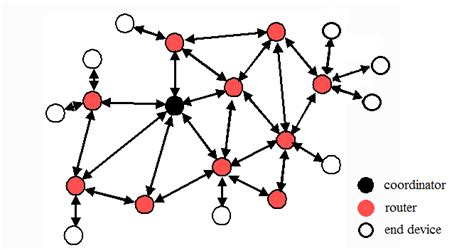
\includegraphics[scale=1]{zigbee_network.png}
\caption{شبکه زیگبی شامل هماهنگ‌کننده، مسیریاب و گره‌پایانی \cite{song2019research}}\label{fig:zigbee_network}
\end{figure}

